\subsection{Sequence Diagrams}

Sequence diagrams illustrate the time-based interactions
between system components, including the client
application, backend services, AI engines,
and database infrastructure.

The sequence diagrams focus on the core workflows
of the aBridgeAI platform, including authentication,
smart content ingestion, Human-in-the-Loop quiz
generation, and context-aware mock interview sessions.
These diagrams emphasize asynchronous processing,
AI integration, and communication across the hybrid
system architecture. The complete set of sequence diagrams
is provided in Appendix~\ref{appendix:sequence-diagrams}.

\noindent\textit{Representative sequence diagrams.} The following diagrams illustrate the authentication flow, smart content ingestion, and HITL quiz generation.

\begin{figure}[H]
	\centering
	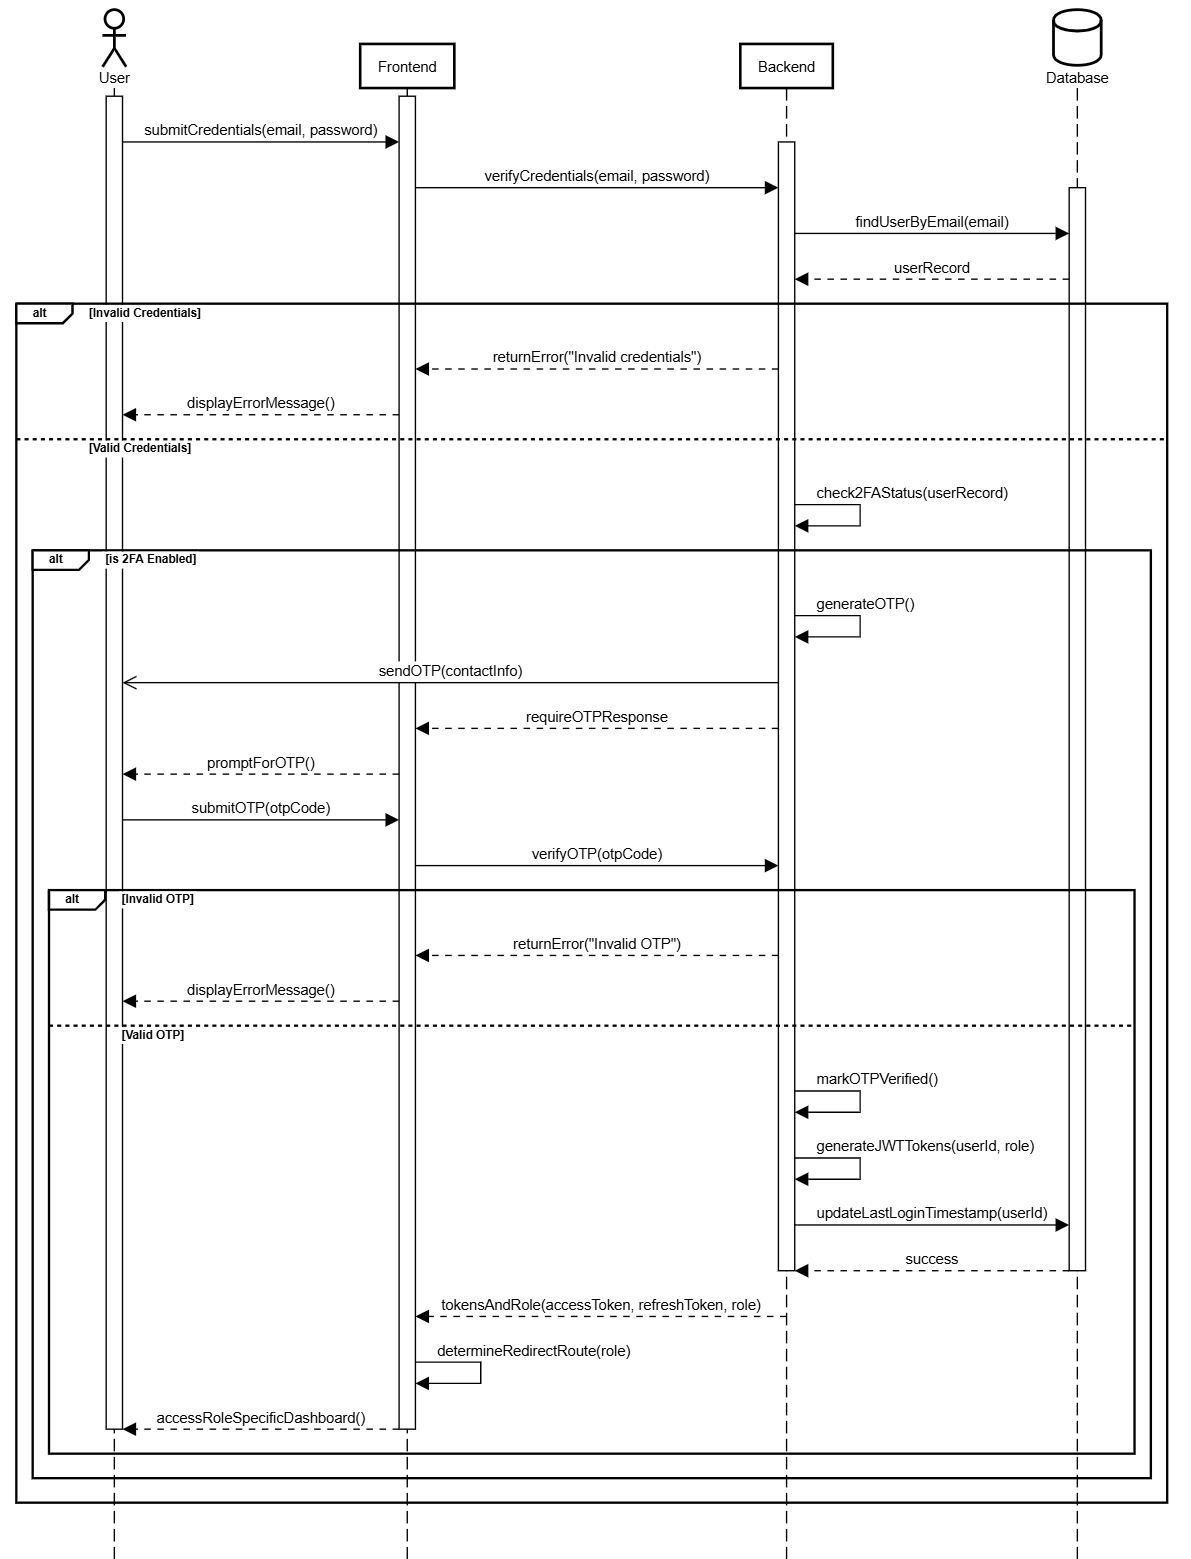
\includegraphics[width=0.95\textwidth]{graphics/seq-diagrams/seq_auth.png}
	\caption{Sequence Diagram: Authentication}
	\label{fig:seq_auth_rep}
\end{figure}

\begin{figure}[H]
	\centering
	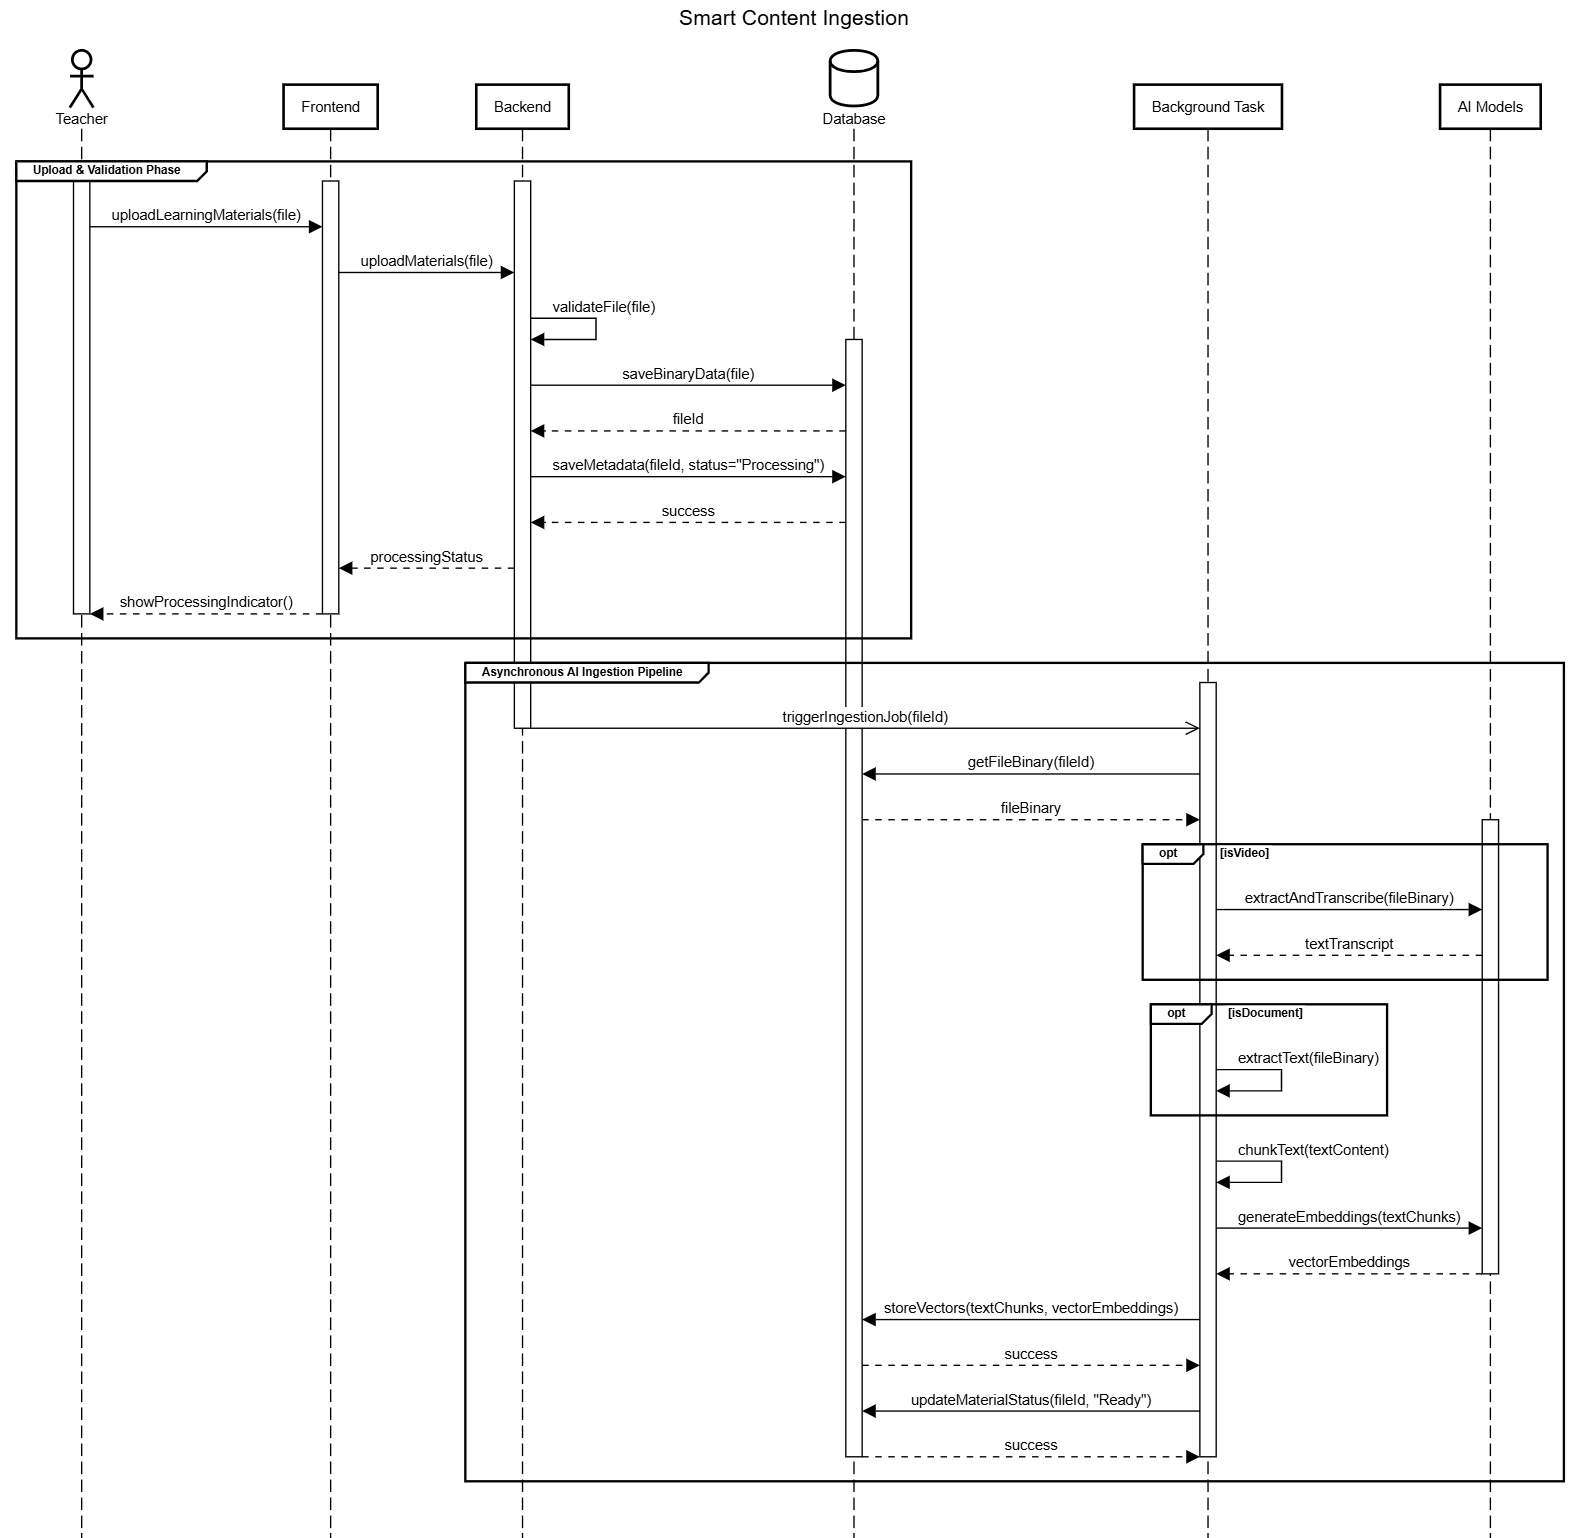
\includegraphics[width=1\textwidth]{graphics/seq-diagrams/seq_ingestion.png}
	\caption{Sequence Diagram: Smart Content Ingestion}
	\label{fig:seq_ingestion_rep}
\end{figure}

\begin{figure}[H]
	\centering
	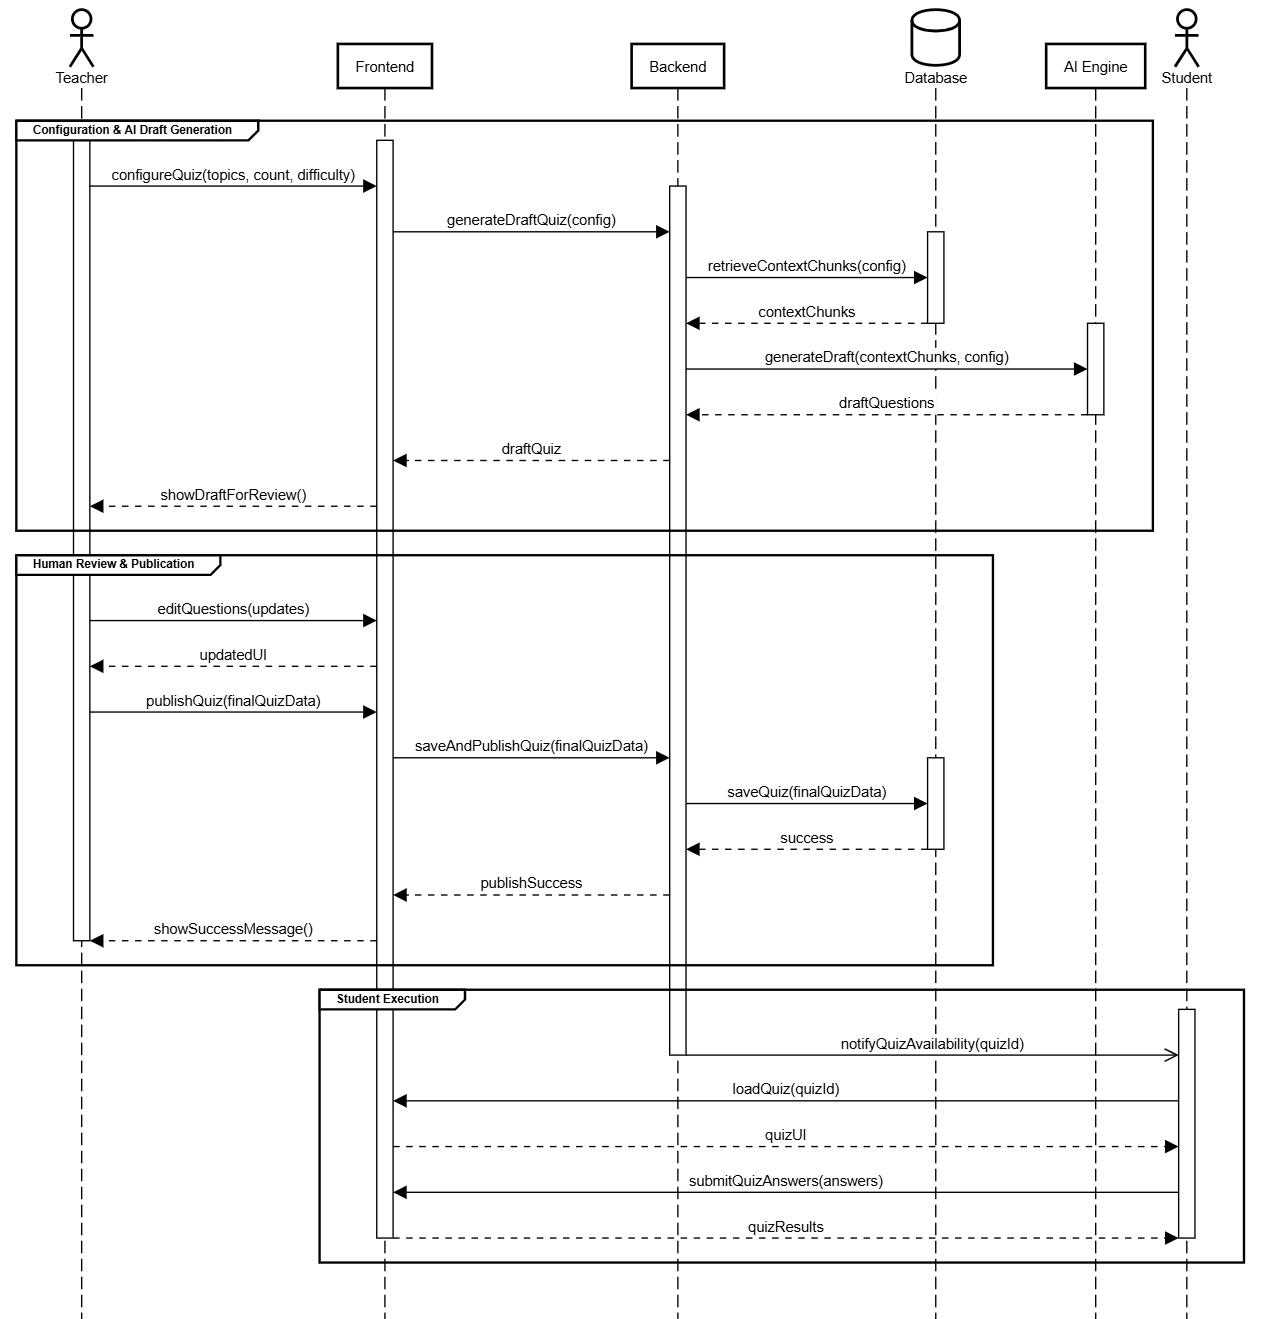
\includegraphics[width=0.95\textwidth]{graphics/seq-diagrams/seq_quiz_gen.png}
	\caption{Sequence Diagram: HITL Quiz Generation and Execution}
	\label{fig:seq_quiz_gen_rep}
\end{figure}

